\chapter{Introducción} 
\label{chap:intro}
\comments{He visto que tienes un glosario, por ahora con pocos
  términos. Te interesa  utilizar glossaries de latex: https://es.sharelatex.com/learn/Glossaries}
\vspace{-0.2cm}

\lsection{Motivación del proyecto}

El derecho a la privacidad en Internet es algo que todo usuario debería valorar y, por desgracia, el gran público no le da la importancia que debería.\\

No son pocas las noticias que están apareciendo últimamente sobre empresas como Google relacionadas con la invasión a la privacidad. Ésto, en gran parte, se ha visto incrementado debido a la llegada de los \textit{smartphones} al mercado(algo relativamente reciente, hace alrededor de 10 años). El poder llevar en nuestro bolsillo todo un ordenador tiene el inconveniente de que grandes empresas como las anteriormente mencionadas pueden tener acceso a información en tiempo real de nosotros, como por ejemplo a la hora a la que nos levantamos, la localización de nuestra propia casa e incluso la ubicación real en todo momento(y sí, de poco sirve deshabilitar la ubicación por GPS en tu smartphone pues también la pueden averiguar mediante el inicio de sesión en una red WiFi).\\
Por otro lado está el tema de las redes sociales. Con el auge de Facebook, Instagram y Twitter, gran parte de la población(en el caso de Norteamérica, casi dos terceras partes) tiene perfil propio en la plataforma Facebook.

\begin{figure}[h]
	\centerline{
		\mbox{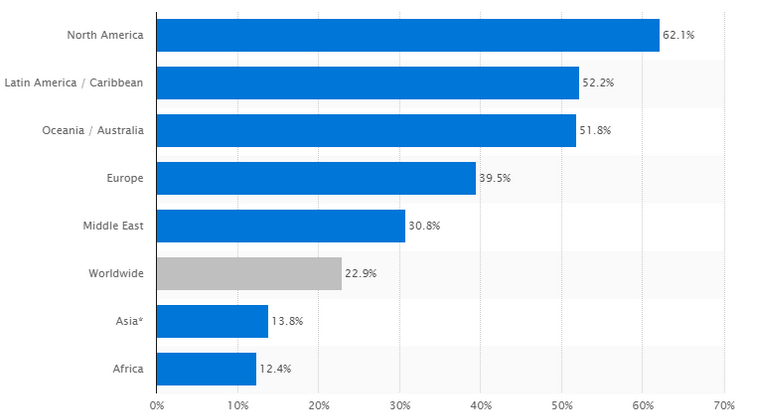
\includegraphics[width=4.00in]{images/sn.png}}
	}
	\caption{Porcentaje de población con perfil en Facebook}
	\label{fig:norm_Daugman}
\end{figure}

Ésto de por sí no es un dato negativo, el problema viene cuando para realizar un registro en una página (como por ejemplo, la web de un diario), la forma más sencilla es conectando con tu perfil personal de Facebook. Ésto causa que, al interaccionar con dicha página(ya sea publicando un comentario, o cualquier tipo de actividad), te arriegues a que aparezca tu nombre real, con todo lo que ello conlleva. Desde este punto, saber todo acerca de ese usuario es tan sencillo como buscar en Google su nombre completo y entrar a su perfil de Facebook, donde aparecen fotos, su dirección, entre otros.\\
En otros casos el iniciar sesión con la cuenta de Google ó Facebook sirve para que dichas empresas conozcan mejor tus gustos y hobbies, para así ofrecerte publicidad a medida. \\

De aquí nace la verdadera motivación de este proyecto. La lucha contra la privacidad en la red es algo que hemos ido perdiendo poco a poco, pero mediante el uso de tecnologías para anonimizarse como las que serán vistas en éste documento se pretende erradicar o, al menos, mitigar éste problema.\\

Parte de la motivación también reside mi interés en el ámbito de la seguridad informática que, desgraciadamente, no está demasiado presente en el temario desarrollado en la carrera. Sin embargo, es un tema de suma importancia y además sirve para poner en práctica metodologías y lenguajes estudiados en el grado. \\

En definitiva, el proyecto  abarca un software modular compuesto de varias herramientas funcionales por sí mismas y donde además el requisito principal es la seguridad del sistema(\textit{security-by-design}).
%bibliografía~\cite{article:Ejemplo}.


\lsection{Objetivos y enfoque}

Principalmente se pretenden lograr dos objetivos fundamentales en este proyecto.\\

El primero es el de hacernos conocedores más a fondo de las diferentes vías a la hora de anonimizarnos en Internet, las variadas herramientas que pretenden conseguir éste objetivo (así como las que pretenden identificar a un usuario), las disparidades entre anonimato y privacidad... En conclusión, realizar una investigación exhaustiva sobre la privacidad en la red.\\

Por otro lado, y quizá el objetivo más importante, es el de poner en práctica los conocimientos adquiridos en la investigación anteriormente dicha. En este caso se ha diseñado, desarrollado y probado una herramienta con numerosas y diversas funciones, cuyo principal propósito es el de garantizarnos una experiencia lo más anónima posible en todo momento.\\


\lsection{Metodología y plan de trabajo}

Éste documento se organiza de la siguiente manera:
\begin{itemize}
	\item Estado  del  Arte: El segundo capítulo explica todos y cada uno de los conceptos de los que trata este proyecto, es decir, el término privacidad, anonimato y la importancia de los mismos hoy en día. Además, se mostrarán ejemplos de herramientas y metodologías para anonimizarse. 
	\item Análisis: El capítulo tres consta de la serie de requisitos, definidos  según  los objetivos  deseados  en  las  aplicaciones  finales  y  delimitados  por  el  alcance  del proyecto.La funcionalidad de la herramienta desarrollada se resume tanto en el catálogo de requisitos como de casos de uso.
	\item Diseño: Este capítulo trata con detalle la fase de diseño, teniendo en cuenta la estructura de la aplicación y el flujo de navegación de la misma 
	\item Desarrollo: En el quinto capítulo se encuentra explicado el método de desarrollo, las librerías utilizadas, los lenguajes en los que está programada la herramienta, las características Software del equipo de desarrollo y el porqué de dicha elección.
	\item Integración, pruebas y resultados: Aquí se tratan las pruebas unitarias realizadas, así como los resultados de las mismas y cómo se han integrado todos los módulos en la aplicación final.
	\item Conclusiones/Trabajo  futuro: Por último, en este capítulo resumimos las conclusiones de la aplicación y el futuro trabajo que se requeriría para que la herramienta vaya creciendo.
\end{itemize}

\newpage \thispagestyle{empty} % Página vacía 